\documentclass[a4paper,12pt]{article}

\usepackage[utf8]{inputenc}
\usepackage[T1]{fontenc}
\usepackage[polish]{babel}
\usepackage{amsmath, amssymb}
\usepackage{graphicx}
\usepackage{geometry}
\usepackage{hyperref}

\geometry{margin=2.5cm}

\title{Planowanie procesu wdrożenia produktu informatycznego za pomocą UML}
\author{Adam Oporski, Kajetan Lach}

\begin{document}

\maketitle

\tableofcontents

\section{Elementy języka UML}
Język UML (Unified Modeling Language) wykorzystuje zestaw graficznych elementów konstrukcyjnych do tworzenia diagramów reprezentujących system. Elementy te są "cegiełkami" modelu i dzielą się głównie na trzy kategorie: strukturalne (opisujące budowę), behawioralne (opisujące zachowanie) oraz grupujące (organizujące model, np. pakiety).

\subsection{Elementy strukturalne}
Elementy strukturalne to "rzeczowniki" języka UML; opisują statyczną architekturę i części składowe systemu. Definiują one, z czego system jest zbudowany, niezależnie od tego, co robi w danym momencie. Do najważniejszych elementów strukturalnych należą:

\begin{figure}[h!]
    \centering
    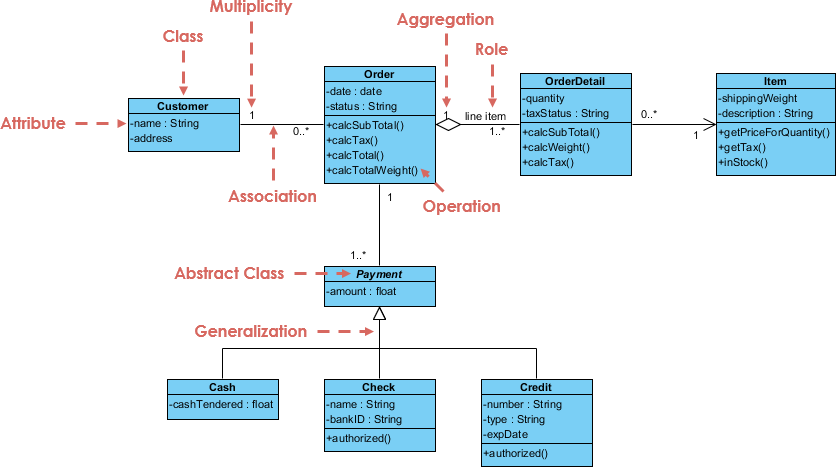
\includegraphics[width=0.8\textwidth]{img/17-class-diagram-example-order-system.png}
\end{figure}

\begin{itemize}
\item Klasa (Class): Szablon do tworzenia obiektów, opisujący ich wspólne atrybuty i operacje.
\item Interfejs (Interface): Zbiór operacji, które klasa musi zaimplementować, definiujący "kontrakt" bez podawania implementacji.
\item Komponent (Component): Modułowa, wymienialna część systemu, która hermetyzuje swoje zachowanie (np. biblioteka .dll).
\item Węzeł (Node): Fizyczny zasób obliczeniowy, na którym uruchamiane jest oprogramowanie (np. serwer, urządzenie).
\item Aktor (Actor): Rola odgrywana przez użytkownika lub inny system zewnętrzny w interakcji z modelowanym systemem.
\end{itemize}

\subsection{Elementy behawioralne}
Elementy behawioralne (zachowaniowe) to "czasowniki" języka UML; opisują dynamiczne aspekty systemu, czyli to, co system robi i jak reaguje w czasie. Koncentrują się na przepływie sterowania i danych. Kluczowe przykłady to:
\begin{itemize}
\item Interakcja (Interaction): Definiuje komunikację między obiektami; jest podstawą diagramów sekwencji i komunikacji.
\item Maszyna stanów (State Machine): Opisuje cykl życia obiektu, pokazując, jak przechodzi on między różnymi stanami w odpowiedzi na zdarzenia.
\item Aktywność (Activity): Reprezentuje przepływ pracy (workflow) lub krok w algorytmie; jest podstawą diagramów aktywności.
\item Przypadek użycia (Use Case): Opisuje sekwencję działań wykonywanych przez system, która przynosi wartość aktorowi (np. "Logowanie użytkownika").
\end{itemize}

\newpage\subsection{Elementy grupujące}
Elementy grupujące to "pudełka" lub "foldery" w języku UML, służące do organizowania modelu. Nie reprezentują one bezpośrednio fizycznej ani logicznej części samego systemu (jak klasa czy komponent), ale pomagają zarządzać jego złożonością, dzieląc model na mniejsze, spójne części.

\begin{figure}[h!]
    \centering
    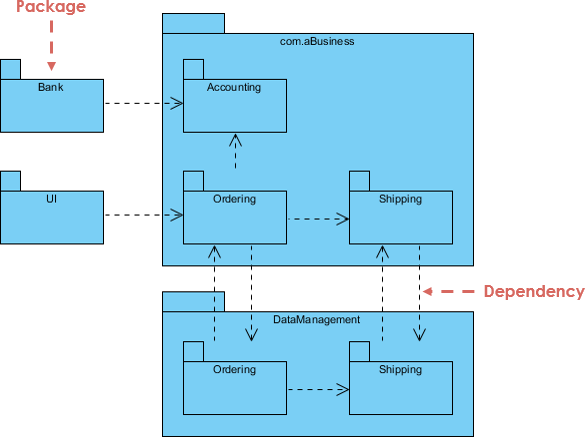
\includegraphics[width=0.8\textwidth]{img/02-simple-package-diagram-example.png}
\end{figure}

\begin{itemize}
\item Pakiet (Package): To podstawowy i najważniejszy element grupujący. Działa jak katalog lub przestrzeń nazw (namespace), która może zawierać dowolne inne elementy UML (klasy, przypadki użycia, komponenty, a nawet inne pakiety).
\item \begin{itemize}
\item Cel: Głównym celem pakietów jest uproszczenie dużych diagramów i całych modeli. Pozwalają one na logiczne podzielenie systemu np. na warstwy (jak "Warstwa prezentacji", "Logika biznesowa", "Dostęp do danych") lub funkcjonalne moduły.
\item Notacja: Zazwyczaj przedstawiany jest jako ikona teczki lub folderu.
\item Widoczność: Pakiety kontrolują również widoczność zawartych w nich elementów, określając, co jest publiczne (widoczne na zewnątrz), a co prywatne (ukryte wewnątrz pakietu).
\end{itemize}
\end{itemize}

\section{Modelowanie wymagań za pomocą przypadków użycia}

Modelowanie przypadków użycia jest kluczową techniką inżynierii oprogramowania, stosowaną we wczesnych fazach projektu do specyfikacji wymagań funkcjonalnych. Celem jest opisanie, w jaki sposób system ma być używany i jakie wartości dostarcza swoim użytkownikom (aktorom). Diagramy przypadków użycia oraz towarzyszące im opisy tekstowe (specyfikacje) stanowią most komunikacyjny między interesariuszami biznesowymi a zespołem deweloperskim, definiując zakres i oczekiwane zachowanie systemu.

\subsection{Kluczowe elementy przypadków użycia}
Model przypadków użycia składa się z kilku fundamentalnych elementów, które razem tworzą spójny obraz funkcjonalności systemu:

\begin{figure}[h!]
    \centering
    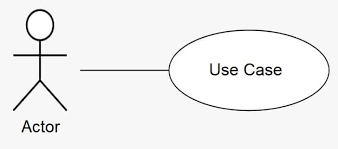
\includegraphics[width=0.8\textwidth]{img/images.png}
\end{figure}


\begin{itemize}
    \item \textbf{Aktor (Actor)}: Reprezentuje rolę odgrywaną przez istotę zewnętrzną wchodzącą w interakcję z systemem. Może to być człowiek (np. "Klient", "Administrator"), inny system komputerowy (np. "System płatności") lub urządzenie (np. "Skaner kodów"). Aktorzy znajdują się \emph{poza} granicami systemu i definiują jego kontekst.

    \item \textbf{Przypadek użycia (Use Case)}: Opisuje sekwencję akcji, jakie system wykonuje, aby dostarczyć konkretną, obserwowalną wartość dla aktora. Jest to jednostka funkcjonalności, np. "Zaloguj użytkownika", "Złóż zamówienie" czy "Wygeneruj raport sprzedaży". Graficznie przedstawiany jako elipsa.

    \item \textbf{Granica systemu (System Boundary)}: Graficznie reprezentowana jako prostokąt, który wizualnie oddziela przypadki użycia (znajdujące się wewnątrz) od aktorów (znajdujących się na zewnątrz). Definiuje ona zakres (scope) modelowanego systemu -- co jest częścią implementacji, a co nią nie jest.

    \item \textbf{Relacje (Relationships)}: Pokazują powiązania między elementami modelu:
    \begin{itemize}
        \item \textbf{Asocjacja (Association)}: Linia ciągła łącząca aktora z przypadkiem użycia. Wskazuje, że aktor uczestniczy w danym przypadku użycia (inicjuje go lub wymienia z nim dane).
        
        \item \textbf{Włączenie (\texttt{<<include>>})}: Relacja stereotypowa (linia przerywana ze strzałką i stereotypem \texttt{<<include>>}) wskazująca, że jeden przypadek użycia (bazowy) \emph{zawsze} i \emph{obowiązkowo} włącza w siebie funkcjonalność innego, mniejszego przypadku (włączanego). Służy do wydzielania wspólnych, powtarzalnych fragmentów (np. "Autoryzuj płatność" włączane do "Złóż zamówienie").
        
        \item \textbf{Rozszerzenie (\texttt{<<extend>>})}: Relacja stereotypowa (linia przerywana ze strzałką i stereotypem \texttt{<<extend>>}) wskazująca, że jeden przypadek użycia (rozszerzający) \emph{może} (ale nie musi) rozszerzyć funkcjonalność przypadku bazowego w określonym punkcie (tzw. punkcie rozszerzenia). Jest to zachowanie opcjonalne, warunkowe (np. "Dodaj kartę podarunkową" rozszerzające "Złóż zamówienie").
        
        \item \textbf{Uogólnienie (Generalization)}: Używane zarówno między aktorami, jak i między przypadkami użycia. Wskazuje, że jeden element (potomny) jest specjalizacją drugiego (nadrzędnego) i dziedziczy jego zachowanie oraz relacje, ale może je modyfikować lub dodawać nowe.
    \end{itemize}

    \item \textbf{Scenariusz (Scenario)}: To konkretna ścieżka wykonania danego przypadku użycia. Każdy przypadek użycia posiada zazwyczaj jeden \textbf{scenariusz główny} (tzw. "happy path", opisujący pomyślny przebieg) oraz wiele \textbf{scenariuszy alternatywnych} i \textbf{wyjątkowych} (opisujących błędy lub alternatywne drogi postępowania).
\end{itemize}

\subsection{Korzyści z modelowania wymagań przez przypadki użycia}

Stosowanie przypadków użycia do specyfikacji wymagań niesie ze sobą liczne korzyści dla procesu wytwórczego oprogramowania:

\begin{itemize}
    \item \textbf{Koncentracja na wartości dla użytkownika}: Przypadki użycia wymuszają myślenie o systemie z perspektywy jego użytkowników i celów, jakie chcą osiągnąć. Gwarantuje to, że implementowane funkcje mają realną wartość biznesową.
    
    \item \textbf{Efektywna komunikacja z interesariuszami}: Diagramy i opisy przypadków użycia są relatywnie łatwe do zrozumienia dla osób nietechnicznych (klientów, menedżerów). Stanowią "wspólny język" i narzędzie do negocjacji oraz walidacji wymagań między biznesem a IT.
    
    \item \textbf{Jasne definiowanie zakresu systemu (Scope)}: Dzięki wizualizacji granicy systemu, model jasno określa, co należy do systemu (i co trzeba zbudować), a co jest jego otoczeniem. Pomaga to w zarządzaniu zakresem projektu i unikaniu jego niekontrolowanego rozrostu (tzw. scope creep).
    
    \item \textbf{Strukturyzacja wymagań}: Pozwalają na dekompozycję złożonego systemu na mniejsze, zarządzalne jednostki funkcjonalności. Relacje \texttt{<<include>>} i \texttt{<<extend>>} pomagają w organizacji i unikaniu redundancji w opisach.
    
    \item \textbf{Fundament dla dalszych etapów projektu}: Przypadki użycia stanowią solidną podstawę wejściową dla:
    \begin{itemize}
        \item \textbf{Projektowania i analizy}: Scenariusze przypadków użycia są bezpośrednim wkładem do tworzenia diagramów interakcji (np. sekwencji) i identyfikacji klas (na diagramach klas).
        \item \textbf{Testowania}: Scenariusze (główny i alternatywne) przekładają się wprost na przypadki testowe (test cases), szczególnie dla testów akceptacyjnych i systemowych.
        \item \textbf{Planowania projektu}: Zbiór przypadków użycia ułatwia estymację pracochłonności, planowanie iteracji (np. w metodykach zwinnych) oraz śledzenie postępu prac.
    \end{itemize}
\end{itemize}

\section{Diagramy czynności i sekwencji}

Diagramy czynności (Activity Diagrams) oraz diagramy sekwencji (Sequence Diagrams) to dwa fundamentalne diagramy behawioralne w języku UML, służące do modelowania dynamicznych aspektów systemu. Chociaż oba opisują zachowanie, robią to z zupełnie różnych perspektyw. 

Diagram czynności koncentruje się na \textbf{przepływie pracy (workflow)} i logice algorytmicznej, pokazując kroki procesu i warunki ich wykonania. 
Diagram sekwencji natomiast koncentruje się na \textbf{interakcjach (komunikatach)} wymienianych między konkretnymi obiektami lub uczestnikami w \textbf{uporządkowaniu czasowym}.

\subsection{Diagram czynności}

Diagram czynności (Activity Diagram) jest w istocie zaawansowanym schematem blokowym (flowchartem). Służy do modelowania przepływu sterowania (control flow) oraz przepływu danych (data flow) z jednej czynności (akcji) do drugiej. Jest idealny do opisywania logiki biznesowej, algorytmów lub kroków realizacji przypadku użycia.

\subsection{Zastosowanie diagramu czynności}

Diagramy czynności są szczególnie użyteczne w następujących sytuacjach:
\begin{itemize}
    \item \textbf{Modelowanie procesów biznesowych (BPM):} Wizualizacja kroków, jakie podejmują różni pracownicy lub działy w organizacji, aby osiągnąć cel biznesowy (np. proces obsługi zamówienia).
    \item \textbf{Opisywanie logiki przypadków użycia:} Przedstawienie szczegółowego scenariusza (głównego lub alternatywnych) dla danego przypadku użycia.
    \item \textbf{Projektowanie algorytmów:} Opisywanie skomplikowanej logiki wewnątrz operacji (metody) klasy, włączając w to pętle, warunki i przetwarzanie równoległe.
    \item \textbf{Wizualizacja przepływów równoległych:} Diagramy te doskonale radzą sobie z pokazywaniem zadań, które mogą lub muszą być wykonywane w tym samym czasie (concurrently).
\end{itemize}

\subsection{Podstawowe elementy diagramu czynności}
\begin{itemize}
    \item \textbf{Węzeł początkowy (Initial Node):} Wypełnione koło. Oznacza początek przepływu.
    \item \textbf{Węzeł końcowy (Activity Final Node):} Wypełnione koło otoczone okręgiem (tzw. "oko byka"). Oznacza koniec całego przepływu.
    \item \textbf{Akcja (Action):} Prostokąt z zaokrąglonymi rogami. Reprezentuje pojedynczy, atomowy krok lub zadanie do wykonania (np. "Oblicz podatek", "Wyślij e-mail").
    \item \textbf{Węzeł decyzyjny (Decision Node):} Romb. Rozdziela przepływ na kilka alternatywnych ścieżek. Każda ścieżka wyjściowa jest opatrzona warunkiem (tzw. "guard condition", np. \texttt{[kwota > 1000]}).
    \item \textbf{Węzeł scalający (Merge Node):} Romb. Łączy kilka alternatywnych ścieżek (pochodzących z węzła decyzyjnego) z powrotem w jeden przepływ.
    \item \textbf{Rozwidlenie (Fork Node):} Gruba, czarna linia (sztabka). Rozdziela jeden przepływ na wiele przepływów równoległych (concurrent flows).
    \item \textbf{Złączenie (Join Node):} Gruba, czarna linia. Synchronizuje przepływy równoległe; czeka, aż wszystkie przepływy wejściowe zostaną zakończone, zanim uruchomi jeden przepływ wyjściowy.
    \item \textbf{Partycje (Partitions / Swimlanes):} Prostokątne obszary (pionowe lub poziome "tory"), które grupują akcje według odpowiedzialności (np. według aktora, działu, komponentu).
\end{itemize}

\subsection{Diagram sekwencji}

Diagram sekwencji (Sequence Diagram) należy do grupy diagramów interakcji. Jego głównym celem jest pokazanie, jak grupa obiektów (uczestników) współpracuje ze sobą, wymieniając komunikaty (wywołując swoje operacje) w określonej kolejności czasowej. Oś czasu biegnie pionowo z góry na dół.

\subsection{Zastosowanie diagramu sekwencji}

Diagramy sekwencji są kluczowe, gdy chcemy:
\begin{itemize}
    \item \textbf{Zrealizować przypadek użycia:} Pokazać, jakie obiekty (klasy) są potrzebne do zrealizowania danego scenariusza przypadku użycia i jak muszą ze sobą "rozmawiać".
    \item \textbf{Zrozumieć logikę kontrolera/serwisu:} Zwizualizować, co dzieje się "pod maską" po wywołaniu jednej metody (np. jakie inne obiekty są wołane, do jakiej bazy danych idzie zapytanie).
    \item \textbf{Zidentyfikować operacje (metody):} Analiza komunikatów wysyłanych do obiektów pomaga w odkrywaniu, jakie publiczne operacje (metody) te obiekty (ich klasy) muszą udostępniać.
    \item \textbf{Projektować interakcje między komponentami:} Modelować komunikację między różnymi częściami systemu, np. między front-endem, API a bazą danych lub między mikroserwisami.
\end{itemize}

\subsection{Podstawowe elementy diagramu sekwencji}
\begin{itemize}
    \item \textbf{Uczestnik / Linia życia (Lifeline):} Reprezentuje pojedynczego uczestnika interakcji (np. instancję klasy \texttt{:SystemBankowy} lub aktora). Graficznie przedstawiony jako prostokąt z pionową, przerywaną linią biegnącą w dół.
    \item \textbf{Pasek aktywacji (Activation Bar):} Cienki, pionowy prostokąt na linii życia. Wskazuje okres, w którym dany obiekt jest aktywny (zajęty), tzn. wykonuje operację (lub czeka na powrót z operacji, którą sam wywołał).
    \item \textbf{Komunikat (Message):} Strzałka łącząca dwie linie życia, reprezentująca komunikację między obiektami.
        \begin{itemize}
            \item \textbf{Komunikat synchroniczny (Synchronous):} Strzałka z pełnym (wypełnionym) grotem. Nadawca wysyła komunikat i czeka na odpowiedź, zanim przejdzie dalej.
            \item \textbf{Komunikat asynchroniczny (Asynchronous):} Strzałka z otwartym grotem (liniowym). Nadawca wysyła komunikat i nie czeka na odpowiedź, kontynuując swoją pracę.
            \item \textbf{Komunikat zwrotny (Reply Message):} Przerywana strzałka. Pokazuje powrót sterowania (i ewentualnie danych) po zakończeniu komunikatu synchronicznego.
        \end{itemize}
    \item \textbf{Fragmenty interakcji (Interaction Fragments):} Prostokątne ramki obejmujące część diagramu, służące do modelowania złożonej logiki:
        \begin{itemize}
            \item \textbf{alt (Alternative):} Modeluje strukturę "if-then-else". Ramka jest podzielona przerywanymi liniami na sekcje, z których każda ma warunek.
            \item \textbf{opt (Optional):} Fragment opcjonalny; wykonuje się tylko wtedy, gdy warunek (guard) jest spełniony (prostsza wersja \textbf{alt}).
            \item \textbf{loop (Loop):} Fragment, który jest wykonywany wielokrotnie, dopóki spełniony jest warunek pętli.
        \end{itemize}
    \item \textbf{Tworzenie (\texttt{<<create>>}) i Niszczenie (Destroy):} Komunikat tworzący nowy obiekt (strzałka wskazująca na prostokąt uczestnika) oraz znak 'X' na końcu linii życia, oznaczający zniszczenie obiektu.
\end{itemize}

\section{Modelowanie klas i powiązań pomiędzy nimi}

Modelowanie klas jest fundamentem projektowania obiektowego. Pozwala ono na statyczne przedstawienie struktury systemu poprzez zdefiniowanie bytów (klas), za które system jest odpowiedzialny, oraz relacji (powiązań) zachodzących między nimi. Diagram klas jest centralnym artefaktem w języku UML, służącym jako plan architektoniczny dla kodu źródłowego.

\subsection{Diagram klas}

Diagram klas (Class Diagram) to statyczny diagram strukturalny, który opisuje budowę systemu poprzez pokazanie jego klas, ich atrybutów, operacji (metod) oraz relacji (powiązań) między tymi klasami. Jest to najczęściej używany i prawdopodobnie najważniejszy diagram UML w kontekście programowania obiektowego (OOP).

Graficznie klasa jest reprezentowana jako prostokąt, zazwyczaj podzielony na trzy sekcje:
\begin{itemize}
    \item \textbf{Nazwa klasy:} Górna sekcja, zawiera nazwę (np. "KontoBankowe").
    \item \textbf{Atrybuty (Attributes):} Środkowa sekcja, zawiera pola lub właściwości klasy (np. "saldo : Pieniadze").
    \item \textbf{Operacje (Operations):} Dolna sekcja, zawiera metody lub funkcje, jakie klasa udostępnia (np. "wplac(kwota : Pieniadze)").
\end{itemize}
Diagram klas pokazuje nie tylko pojedyncze klasy, ale przede wszystkim sposób, w jaki łączą się one w spójny system za pomocą różnych typów relacji (asocjacji, agregacji, kompozycji, dziedziczenia).

\subsection{Zastosowanie diagramu klas}

Diagram klas jest wszechstronnym narzędziem wykorzystywanym na różnych etapach cyklu życia oprogramowania i do różnych celów:

\begin{itemize}
    \item \textbf{Analiza domeny (Domain Modeling):} We wczesnej fazie projektu diagram klas służy do modelowania kluczowych pojęć (bytów) z dziedziny problemu (np. w systemie bankowym będą to "Klient", "Konto", "Transakcja"). Pomaga to analitykom i deweloperom zrozumieć świat biznesu.
    
    \item \textbf{Projektowanie systemu (System Design):} Jest to podstawowe zastosowanie. Deweloperzy używają diagramów klas do projektowania architektury oprogramowania. Decydują, jakie klasy będą potrzebne, jakie będą miały atrybuty i operacje oraz jak będą ze sobą współpracować.
    
    \item \textbf{Generowanie kodu (Code Generation):} Wiele narzędzi typu CASE (Computer-Aided Software Engineering) potrafi automatycznie wygenerować szkielety kodu (np. w Javie, C\#, C++) bezpośrednio z diagramu klas.
    
    \item \textbf{Inżynieria wsteczna (Reverse Engineering):} Narzędzia potrafią również analizować istniejący kod źródłowy i generować z niego diagramy klas. Jest to niezwykle przydatne do zrozumienia i dokumentowania starszych (legacy) systemów.
    
    \item \textbf{Dokumentacja techniczna:} Diagram klas stanowi precyzyjny i jednoznaczny "plan" systemu, który jest łatwiejszy do zrozumienia niż przeglądanie tysięcy linii kodu. Służy jako kluczowy element dokumentacji architektonicznej.
    
    \item \textbf{Komunikacja w zespole:} Diagramy te stanowią wspólny język wizualny dla programistów, projektantów i analityków, ułatwiając dyskusje na temat struktury i odpowiedzialności poszczególnych modułów systemu.
\end{itemize}

\section{Diagramy komponentów}

Diagram komponentów jest statycznym diagramem strukturalnym, który koncentruje się na fizycznym aspekcie systemu. Pokazuje on, jak system jest podzielony na modułowe, wymienialne części (komponenty) oraz jakie są między nimi zależności. Jest to spojrzenie na architekturę systemu z perspektywy modułów kodu i ich powiązań.

\subsection{Zastosowanie diagramu komponentów}

Diagramy te są używane do:
\begin{itemize}
    \item \textbf{Modelowania architektury oprogramowania:} Pokazania głównych "klocków" (modułów, bibliotek, plików wykonywalnych) i ich wzajemnych zależności.
    \item \textbf{Projektowania systemów rozproszonych:} Definiowania usług (np. mikroserwisów) i kontraktów (interfejsów), przez które się komunikują.
    \item \textbf{Zarządzania zależnościami:} Jasnego określenia, które części systemu zależą od których, co jest kluczowe dla utrzymania i rozwoju oprogramowania.
    \item \textbf{Planowania ponownego użycia:} Identyfikacji części systemu, które są na tyle niezależne, że mogą być ponownie wykorzystane w innych projektach.
\end{itemize}

\subsection{Podstawowe elementy diagramu komponentów}
\begin{itemize}
    \item \textbf{Komponent (Component):} Logiczna, modułowa część systemu, która hermetyzuje swoje zachowanie i jest wymienialna. Graficznie przedstawiany jako prostokąt ze stereotypem \texttt{<<component>>} lub ikoną (prostokąt z dwoma mniejszymi prostokątami na boku).
    \item \textbf{Interfejs (Interface):} "Kontrakt" definiujący zbiór operacji, które komponent dostarcza (realizuje) lub których wymaga od innych komponentów.
        \begin{itemize}
            \item \textbf{Interfejs realizowany (Provided):} Oznaczany jako "lizak" (kółko na końcu linii ciągłej). Pokazuje, co komponent oferuje światu.
            \item \textbf{Interfejs wymagany (Required):} Oznaczany jako "gniazdko" (półkole na końcu linii ciągłej). Pokazuje, czego komponent potrzebuje do działania.
        \end{itemize}
    \item \textbf{Port (Port):} Mały kwadrat na granicy komponentu, reprezentujący punkt interakcji. Interfejsy są często "podłączone" do portów.
    \item \textbf{Zależność (Dependency):} Linia przerywana ze strzałką, pokazująca, że jeden komponent (klient) zależy od innego (dostawcy).
\end{itemize}

\section{Podział modelu na pakiety}

Podział na pakiety jest podstawowym mechanizmem organizacyjnym w UML. Służy do grupowania powiązanych ze sobą elementów modelu (np. klas, przypadków użycia, komponentów) w spójne jednostki, podobnie jak katalogi grupują pliki w systemie operacyjnym lub przestrzenie nazw (namespaces) w językach programowania.

\subsection{Diagram pakietów}

Diagram pakietów (Package Diagram) to diagram strukturalny, którego głównym celem jest pokazanie, jak model jest zorganizowany w pakiety oraz jakie są zależności między tymi pakietami. Upraszcza on złożone diagramy (np. diagramy klas) poprzez ukrycie szczegółów i pokazanie widoku "z lotu ptaka" na architekturę systemu.

\subsection{Podstawowe elementy diagramu pakietów}
\begin{itemize}
    \item \textbf{Pakiet (Package):} Podstawowy element grupujący. Przedstawiany graficznie jako ikona teczki (folderu). Może zawierać inne elementy, w tym inne pakiety (zagnieżdżenie).
    \item \textbf{Zależność (Dependency):} Linia przerywana ze strzałką. Wskazuje, że co najmniej jeden element w pakiecie klienta zależy od co najmniej jednego elementu w pakiecie dostawcy.
    \item \textbf{Stereotypy zależności:}
        \begin{itemize}
            \item \textbf{\texttt{<<import>>}:} Wskazuje, że zawartość pakietu docelowego jest dodawana do przestrzeni nazw pakietu źródłowego (jak \texttt{using} w C\# lub \texttt{import} w Javie).
            \item \textbf{\texttt{<<access>>}:} Wskazuje, że pakiet źródłowy ma dostęp do zawartości pakietu docelowego, ale jej nie importuje (dostęp wymaga kwalifikacji nazwy).
        \end{itemize}
    \item \textbf{Scalanie pakietów (Package Merge):} Relacja wskazująca, że zawartość jednego pakietu jest łączona z zawartością drugiego, rozszerzając go.
\end{itemize}

\section{Modelowanie wdrożenia systemu}

Modelowanie wdrożenia (deployment) dotyczy fizycznej, uruchomieniowej architektury systemu. Odpowiada na pytania: "Jakie mamy zasoby sprzętowe (serwery, urządzenia)?" oraz "Gdzie (na jakim sprzęcie) zostaną uruchomione poszczególne komponenty oprogramowania?".

\subsection{Diagram wdrożenia}

Diagram wdrożenia (Deployment Diagram) jest statycznym diagramem strukturalnym, który wizualizuje fizyczną topologię systemu. Przedstawia węzły (zasoby sprzętowe lub środowiska uruchomieniowe) oraz artefakty (oprogramowanie), które są na nich wdrażane (instalowane, uruchamiane).

\subsection{Podstawowe elementy diagramu wdrożenia}
\begin{itemize}
    \item \textbf{Węzeł (Node):} Zasób obliczeniowy zdolny do uruchamiania oprogramowania. Graficznie przedstawiany jako trójwymiarowy sześcian (kostka).
        \begin{itemize}
            \item \textbf{Węzeł urządzenia (Device Node):} Fizyczny sprzęt, np. "Serwer Aplikacji", "Komputer Kliencki".
            \item \textbf{Węzeł środowiska uruchomieniowego (Execution Environment Node):} Oprogramowanie służące do hostowania innego oprogramowania, np. "Serwer JVM", "Kontener Docker".
        \end{itemize}
    \item \textbf{Artefakt (Artifact):} Fizyczny produkt procesu wytwórczego, np. plik \texttt{.jar}, \texttt{.dll}, plik wykonywalny \texttt{.exe}, skrypt SQL. Graficznie przedstawiany jako prostokąt ze stereotypem \texttt{<<artifact>>} lub ikoną dokumentu z zagiętym rogiem.
    \item \textbf{Relacja wdrożenia (Deployment):} Linia przerywana ze strzałką i stereotypem \texttt{<<deploy>>}, łącząca artefakt z węzłem, na którym jest on wdrażany.
    \item \textbf{Ścieżka komunikacyjna (Communication Path):} Linia ciągła łącząca dwa węzły. Reprezentuje fizyczne lub logiczne połączenie sieciowe (np. "HTTP", "JDBC", "Ethernet"), przez które węzły się komunikują.
\end{itemize}

\section{Visual Paradigm online - opis działania i alternatywy}

Modelowanie UML wymaga wsparcia narzędziowego (tzw. narzędzi CASE - Computer-Aided Software Engineering). Na rynku dostępnych jest wiele rozwiązań, od prostych edytorów graficznych po zintegrowane platformy modelistyczne.

\subsection{Visual Paradigm Online (VP Online)}

Jest to popularna, webowa (działająca w chmurze) platforma do modelowania.
\begin{itemize}
    \item \textbf{Działanie:} Działa w przeglądarce internetowej. Oferuje bogaty zestaw palet i narzędzi do tworzenia diagramów zgodnych ze standardem UML. Poza UML wspiera także inne notacje (np. BPMN dla procesów biznesowych, ArchiMate dla architektury korporacyjnej, diagramy ERD dla baz danych).
    \item \textbf{Cechy:} Kładzie silny nacisk na współpracę (współdzielenie diagramów, komentowanie), integrację (np. z G Suite, Office 365) oraz posiada pewne zaawansowane funkcje, jak generowanie dokumentacji.
    \item \textbf{Model biznesowy:} Dostępny jest w modelu freemium. Wersja darmowa oferuje podstawową funkcjonalność, natomiast pełne możliwości (np. generowanie kodu, praca zespołowa) są dostępne w płatnych subskrypcjach.
\end{itemize}

\subsection{Draw.io (obecnie diagrams.net)}

Jest to darmowe i niezwykle popularne narzędzie do tworzenia wszelkiego rodzaju diagramów, działające online lub jako aplikacja desktopowa.
\begin{itemize}
    \item \textbf{Działanie:} Jest to przede wszystkim edytor grafiki wektorowej, a nie dedykowane narzędzie CASE. Oznacza to, że oferuje szablony (kształty) dla UML, ale nie "rozumie" semantyki modelu. Nie waliduje poprawności połączeń ani nie potrafi generować kodu na podstawie diagramu klas.
    \item \textbf{Zastosowanie:} Idealne do szybkiego szkicowania, tworzenia prostych diagramów na potrzeby dokumentacji lub prezentacji. Jego największą zaletą jest prostota, zerowy koszt i doskonała integracja z narzędziami takimi jak Confluence, Jira czy Google Drive.
    \item \textbf{Alternatywa dla VP:} Jest świetną alternatywą, jeśli potrzebujemy tylko narysować diagram, a nie zarządzać złożonym, spójnym modelem systemu.
\end{itemize}

\section{Wnioski}

\subsection{Potencjalne przypadki użycia UML}

UML jest językiem uniwersalnym, który znajduje zastosowanie w wielu obszarach inżynierii oprogramowania:
\begin{itemize}
    \item \textbf{Zbieranie wymagań:} Diagramy przypadków użycia do komunikacji z klientem.
    \item \textbf{Analiza biznesowa:} Diagramy czynności do modelowania procesów biznesowych (workflow).
    \item \textbf{Projektowanie architektury:} Diagramy komponentów i pakietów do definicji struktury wysokiego poziomu.
    \item \textbf{Projektowanie szczegółowe:} Diagramy klas (struktura danych) i sekwencji (logika interakcji) jako plan dla programistów.
    \item \textbf{Modelowanie wdrożenia:} Diagramy wdrożenia do planowania infrastruktury.
    \item \textbf{Dokumentacja i inżynieria wsteczna:} Tworzenie diagramów z istniejącego kodu, aby ułatwić jego zrozumienie i utrzymanie.
\end{itemize}

\subsection{Potencjalne problemy z używaniem UML}

Mimo swoich zalet, UML bywa krytykowany, a jego nieprawidłowe użycie prowadzi do problemów:
\begin{itemize}
    \item \textbf{Nadmierne modelowanie (Over-modeling):} Tworzenie zbyt wielu diagramów, które są zbyt szczegółowe. Zespół spędza więcej czasu na rysowaniu niż na tworzeniu działającego oprogramowania.
    \item \textbf{Paraliż analityczny (Analysis Paralysis):} Ciągłe udoskonalanie modeli bez przechodzenia do fazy implementacji.
    \item \textbf{Dezaktualizacja diagramów:} Największy problem. Diagramy są tworzone na początku, ale kod ewoluuje. Jeśli diagramy nie są aktualizowane równolegle z kodem, stają się bezużyteczne, a nawet szkodliwe (wprowadzają w błąd).
    \item \textbf{Złożoność języka:} UML jest duży (14 typów diagramów). Zespoły często znają tylko podstawy (diagramy klas i przypadków użycia), co ogranicza jego potencjał.
    \item \textbf{Bariera komunikacyjna:} Zbyt skomplikowane diagramy mogą być niezrozumiałe dla interesariuszy biznesowych, niwecząc cel komunikacyjny.
\end{itemize}

\subsection{Podsumowanie}

UML (Unified Modeling Language) pozostaje kluczowym standardem w inżynierii oprogramowania. Nie jest to metodologia, lecz \textbf{język} -- zestaw narzędzi notacyjnych do wizualizacji, specyfikacji, konstruowania i dokumentowania systemów.

Wartość UML nie leży w samych diagramach, ale w \textbf{myśleniu projektowym} i \textbf{komunikacji}, którą one umożliwiają. W nowoczesnych, zwinnych (Agile) metodykach odchodzi się od tworzenia kompletnej, szczegółowej dokumentacji UML "na zapas" (Big Design Up Front). Zamiast tego, UML jest używany w sposób pragmatyczny i "w sam raz" (just-enough modeling), do rozwiązywania konkretnych problemów projektowych lub wyjaśniania złożonych interakcji w zespole, często na tablicy, a niekoniecznie w skomplikowanym narzędziu CASE.

\end{document}
